%% start of file `template.tex'.
%% Copyright 2006-2015 Xavier Danaux (xdanaux@gmail.com).
%
% This work may be distributed and/or modified under the
% conditions of the LaTeX Project Public License version 1.3c,
% available at http://www.latex-project.org/lppl/.


\documentclass[11pt,a4paper,sans]{moderncv}        % possible options include font size ('10pt', '11pt' and '12pt'), paper size ('a4paper', 'letterpaper', 'a5paper', 'legalpaper', 'executivepaper' and 'landscape') and font family ('sans' and 'roman')
\usepackage{ragged2e}
\usepackage{lastpage}
\usepackage[german]{babel} 
\usepackage{fancyhdr}

\fancyfoot[C]{ \thepage\ / \pageref{LastPage}}
\usepackage{pdfpages}
% moderncv themes
\moderncvstyle{classic}                             % style options are 'casual' (default), 'classic', 'banking', 'oldstyle' and 'fancy'
\moderncvcolor{blue}                               % color options 'black', 'blue' (default), 'burgundy', 'green', 'grey', 'orange', 'purple' and 'red'
%\renewcommand{\familydefault}{\sfdefault}         % to set the default font; use '\sfdefault' for the default sans serif font, '\rmdefault' for the default roman one, or any tex font name
%\nopagenumbers{}                                  % uncomment to suppress automatic page numbering for CVs longer than one page

% character encoding
%\usepackage[utf8]{inputenc}                       % if you are not using xelatex ou lualatex, replace by the encoding you are using
%\usepackage{CJKutf8}                              % if you need to use CJK to typeset your resume in Chinese, Japanese or Korean

% adjust the page margins
\usepackage[scale=0.75]{geometry}
%\setlength{\hintscolumnwidth}{3cm}                % if you want to change the width of the column with the dates
%\setlength{\makecvtitlenamewidth}{10cm}           % for the 'classic' style, if you want to force the width allocated to your name and avoid line breaks. be careful though, the length is normally calculated to avoid any overlap with your personal info; use this at your own typographical risks...

% personal data
\name{Fabian E.}{Gruber}
%\title{Resumé title}                               % optional, remove / comment the line if not wanted
\address{Anna-Stainer-Knittel-Weg 3/5/4}{6020 Innsbruck, \"Osterreich}% optional, remove / comment the line if not wanted; the "postcode city" and "country" arguments can be omitted or provided empty
\phone[mobile]{+43~650~2587521}                   % optional, remove / comment the line if not wanted; the optional "type" of the phone can be "mobile" (default), "fixed" or "fax"
%\phone[fixed]{+2~(345)~678~901}
%\phone[fax]{+3~(456)~789~012}
\email{Fabian.Gruber@uibk.ac.at}                               % optional, remove / comment the line if not wanted
%\homepage{www.johndoe.com}                         % optional, remove / comment the line if not wanted
%\social[linkedin]{john.doe}                        % optional, remove / comment the line if not wanted
%\social[twitter]{jdoe}                             % optional, remove / comment the line if not wanted
%\social[github]{jdoe}                              % optional, remove / comment the line if not wanted
%\extrainfo{additional information}                 % optional, remove / comment the line if not wanted
\photo[64pt][0.2pt]{IMG_3890_cropped2}                       % optional, remove / comment the line if not wanted; '64pt' is the height the picture must be resized to, 0.4pt is the thickness of the frame around it (put it to 0pt for no frame) and 'picture' is the name of the picture file
%\quote{}                                 % optional, remove / comment the line if not wanted

% bibliography adjustements (only useful if you make citations in your resume, or print a list of publications using BibTeX)
%   to show numerical labels in the bibliography (default is to show no labels)
\makeatletter\renewcommand*{\bibliographyitemlabel}{\@biblabel{\arabic{enumiv}}}\makeatother
%   to redefine the bibliography heading string ("Publications")
%\renewcommand{\refname}{Articles}

% bibliography with mutiple entries
%\usepackage{multibib}
%\newcites{book,misc}{{Books},{Others}}
%----------------------------------------------------------------------------------
%            content
%----------------------------------------------------------------------------------
\begin{document}
%\begin{CJK*}{UTF8}{gbsn}                          % to typeset your resume in Chinese using CJK

%-----       letter       ---------------------------------------------------------
% recipient data
\recipient{SynerGIS Informationssysteme GmbH \\z.H. Herrn Gernot Tutsch}{Technologiestra{\ss}e 10\\1120 Wien}
\date{15. Dezember 2017}
\opening{Sehr geehrter Herr Tutsch!}
\closing{Mit besten Gr\"{u}{\ss}en,}
\enclosure[Anhang]{Lebenslauf, Publikationsliste, Diplombescheid und Zeugnis der zweiten Diplompr\"ufung}       % use an optional argument to use a string other than "Enclosure", or redefine \enclname

\makelettertitle
\justify
Ich m\"ochte mich hiermit f\"ur die Stelle des GIS Team Mitarbeiters bewerben.

Als wissenschaftlicher Mitarbeiter an der Leopold Franzens Universitat (LFU) Innsbruck am Institut f\"ur Geographie bin ich im Moment im Rahmen des Projekts \emph{Shallow erosion dynamics in mountain grasslands of South Tyrol: Monitoring, process analysis and mitigation measures (EroDyn)} angestellt und schreibe an meiner Dissertation mit dem Titel \emph{Digital terrain analysis to support field soil survey}. Darin untersuche ich z.B. mit Methoden des maschinellen Lernens ob automatisierte Gel\"andeklassifikationen mit dem Landschaftsbild von Bodenkartierern \"ubereinstimmen oder wie Oberfl\"achenrauhigkeiten zur Charakterisierung geologischer Einheiten verwendet werden k\"onnen.

Erfahrungen mit GIS sammle ich bereits seit meinem Studium der Kulturtechnik und Wasserwirtschaft an der Universit\"at f\"ur Bodenkultur in Wien. In dieser Zeit verwendete ich vorwiegend ArcGIS, etwa als Tutor f\"ur Mitstudenten, aber auch als studentischer Mitarbeiter sowie sp\"ater als wissenschaftlicher Projektmitarbeiter bei der Kartierung von Landbedeckungsklassen sowie Naturgefahrenereignissen und deren r\"aumlicher Modellierung. Hier machte ich auch erste Schritte in der statistischen Analyse r\"aumlicher Daten mit   R, der freien Programmiersprache f\"{u}r statistisches Rechnen. 



Die intensive Besch\"aftigung mit Open Source GIS hat mir, wenn auch nicht ArcGIS-spezifisch, wichtige Einblicke in die Funktionsweise von GIS im Allgemeinen sowie darin integrierten  spezifischen Tools gebracht. Meine Python-Grundlagen erlauben mir neben der Automatisierung von Abl\"aufen zur L\"osung spezifischer, vor allem raumbezogener Aufgaben auch Einsicht in den Code vieler GIS-Tools zu nehmen und die tats\"achlichen Berechnungen besser zu verstehen. Aufgrund meiner langj\"{a}hrigen Erfahrung als Projektmitarbeiter an verschiedenen Universit\"{a}ten bin ich mit selbstst\"andigem Arbeiten ebenso vertraut wie mit der Zusammenarbeit mit Personen aus unterschiedlichsten Fachgebieten. Meine Lernbereitschaft zeigt sich zum einen in der selbstst\"andigen Einarbeitung in neue Themen und Software im Rahmen meiner Forschungst\"atigkeiten sowie zum anderen in der freiwilligen Teilnahme und  Absolvierierung von Onlinekursen wie z.B. \emph{Statistical learning} von Stanford Online oder \emph{Echoes in Space - Introduction to radar remote sensing} der European Space Agency. Dies unterstreicht mein ausgepr\"agtes Interesse an Geoinformation und verwandten Bereichen. Die Arbeit als Lektor im Fach \emph{\"Ubungen zur Statistik} zeigt au{\ss}erdem mein Interesse selbst angeeignetes Wissen weiter zu geben.

Nach mehreren Jahren der T\"atigkeit an Universit\"aten m\"ochte ich nun ein neues Kapitel aufschlagen und mich f\"ur die ausgeschriebene Stelle als Mitarbeiter des GIS Teams bewerben. An der Stelle reizt mich sowohl die M\"oglichkeit, mich auch in Zukunft intensiv mit GIS besch\"aftigen zu k\"onnen, als auch  Kunden bei der Analyse und L\"osung von spezifischen Problemen zu unterst\"utzen .

\"Uber eine Einladung zu einem Gespr\"ach w\"urde ich mich freuen.

\makeletterclosing
\clearpage
%-----       resume       ---------------------------------------------------------
\makecvtitle


\section{Berufserfahrung}
\cventry{2013--heute   }{Wissenschaftlicher Mitarbeiter}{Institut f\"{u}r Geographie, Universit\"{a}t Innsbruck}{Innsbruck}{}{Forschungsprojekte: 
\begin{itemize}%
\item \emph{Shallow erosion dynamics in mountain grasslands of South Tyrol: Monitoring, process analysis and mitigation measures (EroDyn)}
  \begin{itemize}%
  \item Geodatenmanagement 
   \item Gel\"{a}ndeklassifizierung f\"{u}r automatisierte Blaikenkartierung
   \item Dispositionskartierung auf Landesebene
   \end{itemize}
\item \emph{ReBo -- Reliefklassifizierung aus ALS Daten als Grundlage f\"ur die Regionalisierung von Bodendaten}
  \begin{itemize}%
  \item Ableitung von Landschaftseinheiten mit maschinellem Lernen und automatisierten Gel\"{a}ndeklassifikationsalgorithmen
  \item Bodenkundliche Feldarbeit
  \item Mitarbeit bei der Entwicklung der Java-Applikation \emph{SEPP} (Soil Evaluation in Planning Procedures) f\"{u}r Bodenfunktionsbewertungen
  \end{itemize}
\end{itemize}}
\cventry{2016--2017}{Universit\"{a}tsdozent}{Institut f\"{u}r Geographie, Universit\"{a}t Innsbruck}{Innsbruck}{}{\"{U}bungen zur Statistik mit R (2 Semester)}
\cventry{2016--2017}{Bildungskarenz}{}{Innsbruck}{}{Arbeit an der Dissertation mit dem Arbeitstitel \emph{Digital terrain analysis to support field soil survey}}
\cventry{2011--2013}{Wissenschaftlicher Mitarbeiter}{Institut f\"{u}r Angewandte Geologie, BOKU}{Wien}{}{Forschungsprojekte: 
\begin{itemize}%
\item \emph{Hazard assessment for an expected dam break flood in the Hunza Valley, Pakistan: A combination of GIS, Remote Sensing, and computer simulation techniques}
\begin{itemize}%
  \item Dammbruch-Modellierung mit BREACH
  \item Hydraulische Modellierung mit FLO-2D
  \end{itemize}
\item \emph{Poverty Alleviation through Mitigation of Integrated High-Mountain Risk (PAMIR)}
\begin{itemize}%
  \item Kartierung von Naturgefahren, Gletschern und Infrastruktur mit GIS und Fernerkundungsmethoden
  \end{itemize}
  \end{itemize}}
\cventry{2009--2010}{Projektmitarbeiter}{Institut f\"{u}r Angewandte Geologie, BOKU}{Wien}{}{Forschungsprojekt: 
\begin{itemize}%
\item \emph{Remote Geohazards Assessment in Tajikistan (TajHaz)}
\begin{itemize}%
  \item Kartierung von Naturgefahren und Gletscherseen anhand von Satellitenbildern  und GIS
  \item Feldarbeit in Tajikistan
  \end{itemize}
  \end{itemize}}

\cventry{2010--2011}{Tutor}{ Institut f\"ur Landschaftsentwicklung, Erholungs- und Naturschutzplanung, BOKU}{Wien}{}{Tutor f\"ur ArcGIS im Rahmen der LV \emph{Einf\"uhrung in GIS}}

\section{Ausbildung}
\cvitem{2002--2011}{Diplomstudium der Kulturtechnik und Wasserwirtschaft an der Universit\"{a}t f\"{u}r Bodenkultur (BOKU), Wien}
\cvitem{1993--2001}{Linz International School Auhof, Linz:
Abschluss mit Matura und International Baccalaureate (IB)}
\cvitem{1991--1993}{Volksschule Linz-Pichling}
\cvitem{1989--1991}{Lincoln Elementary School Pittsburgh, PA, USA}

\section{Diplomarbeit}
\cvitem{Titel}{\emph{The 2010 Attabad Landslide Dam Lake:
modeling and prediction of Lake Outburst
Floods}}
\cvitem{Betreuer}{Jean F. Schneider und Martin Mergili}

\section{Sprachen}
\cvitemwithcomment{Deutsch}{Muttersprache}{ }
\cvitemwithcomment{Englisch}{Verhandlungssicher}{ }
\cvitemwithcomment{Spanisch}{Grundkenntnisse}{ }
\cvitemwithcomment{Franz\"osisch}{Grundkenntnisse}{ }

\section{EDV-Kenntnisse}
\cvdoubleitem{Operating systems}{Linux (Ubuntu), Windows} {Languages}{R, Python, Bash}
\cvdoubleitem{Geographic information systems}{ArcGIS, GRASS, SAGA, QGIS } {Text- verarbeitung } {MS Word, Libreoffice,  \LaTeX{} with Texmaker}
\cvdoubleitem{Bild- verarbeitung}{GIMP, Inkscape} {Modellierungs- software } {FLO-2D, Ramms, Dan-3D}
\section{Hobbies}
\cvitem{G\"artnerei}{Mitarbeit beim Gemeinschaftsgarten der Vinzigemeinschaft Waldhuttl, Innsbruck}
\cvitem{Reisen}{Reisen durch Mittel- und S\"udamerika, Zentralasien, S\"udostasien und Madagaskar}


\clearpage
%\clearpage\end{CJK*}                              % if you are typesetting your resume in Chinese using CJK; the \clearpage is required for fancyhdr to work correctly with CJK, though it kills the page numbering by making \lastpage undefined
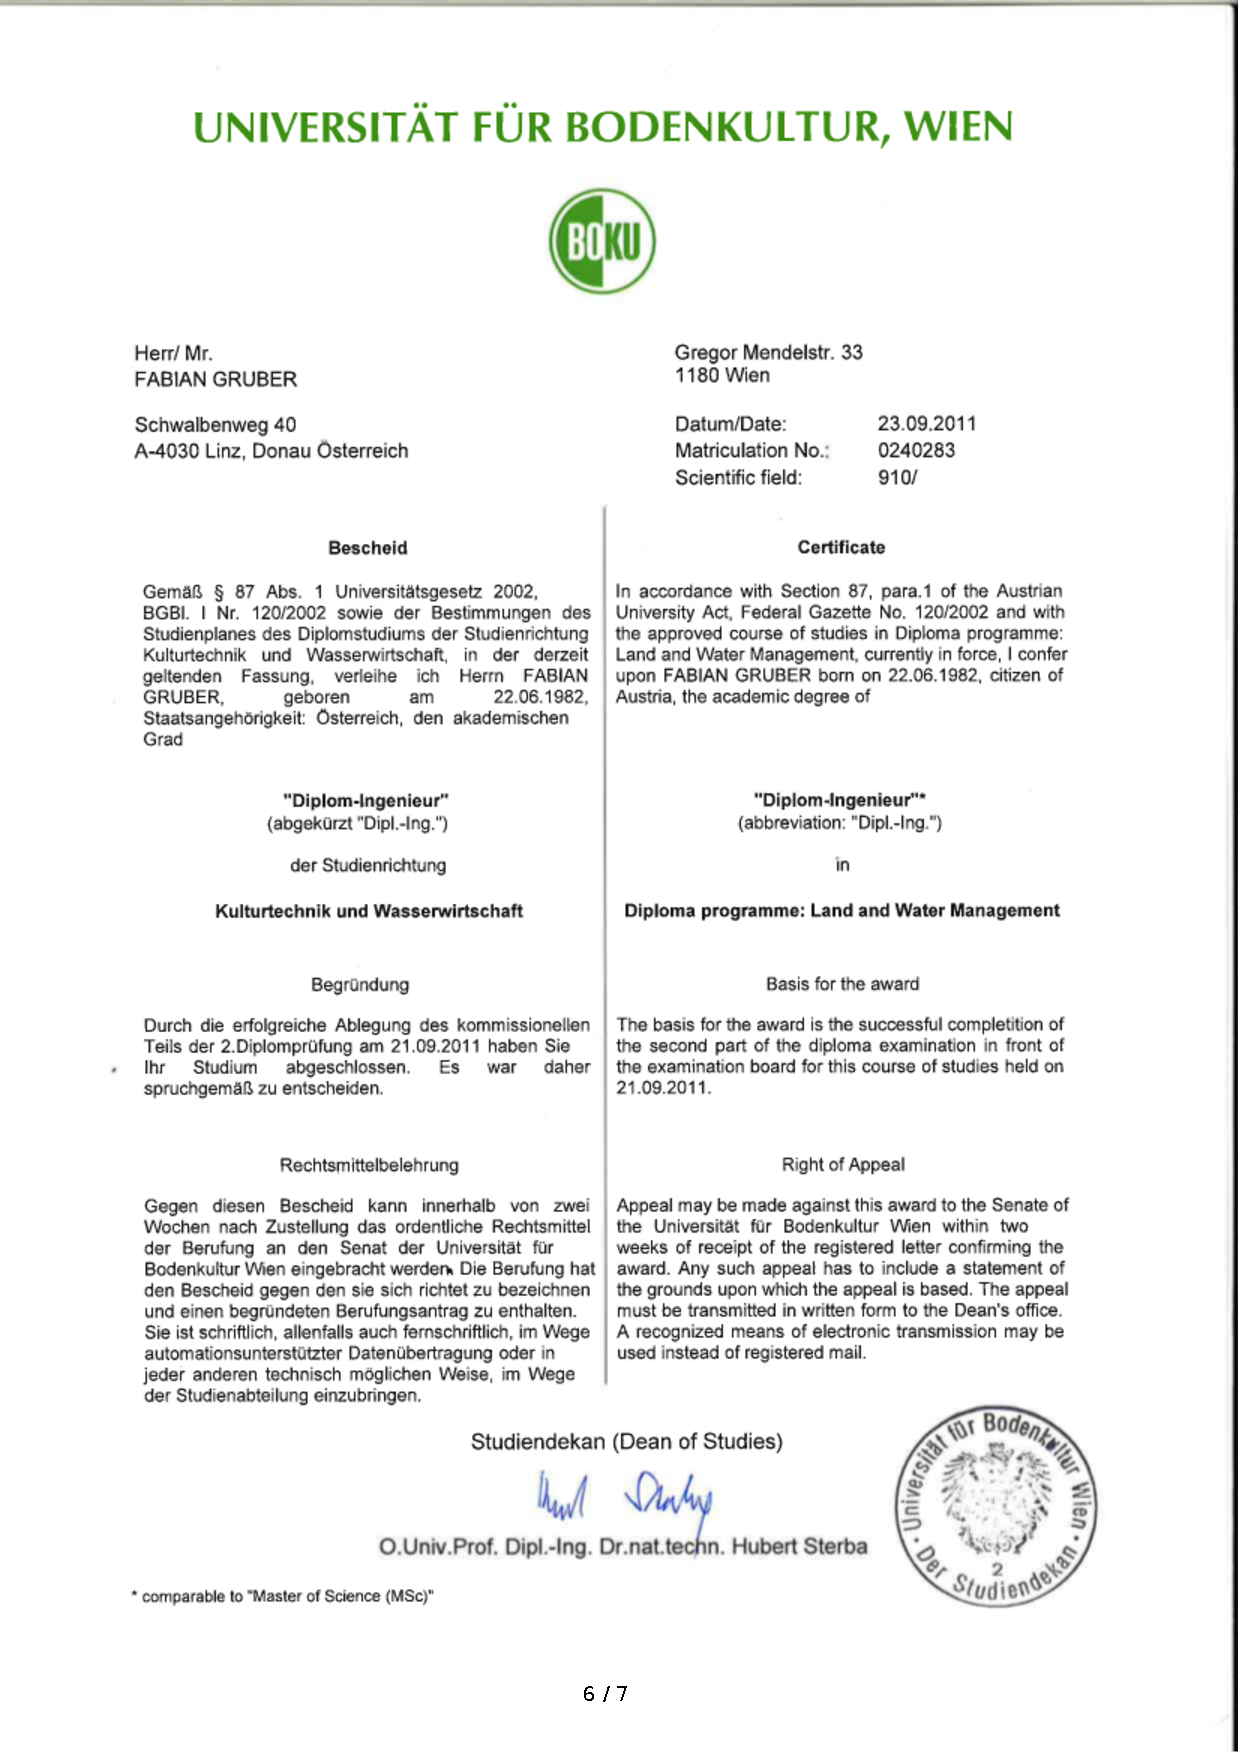
\includepdf{DP_seite6von7.pdf}
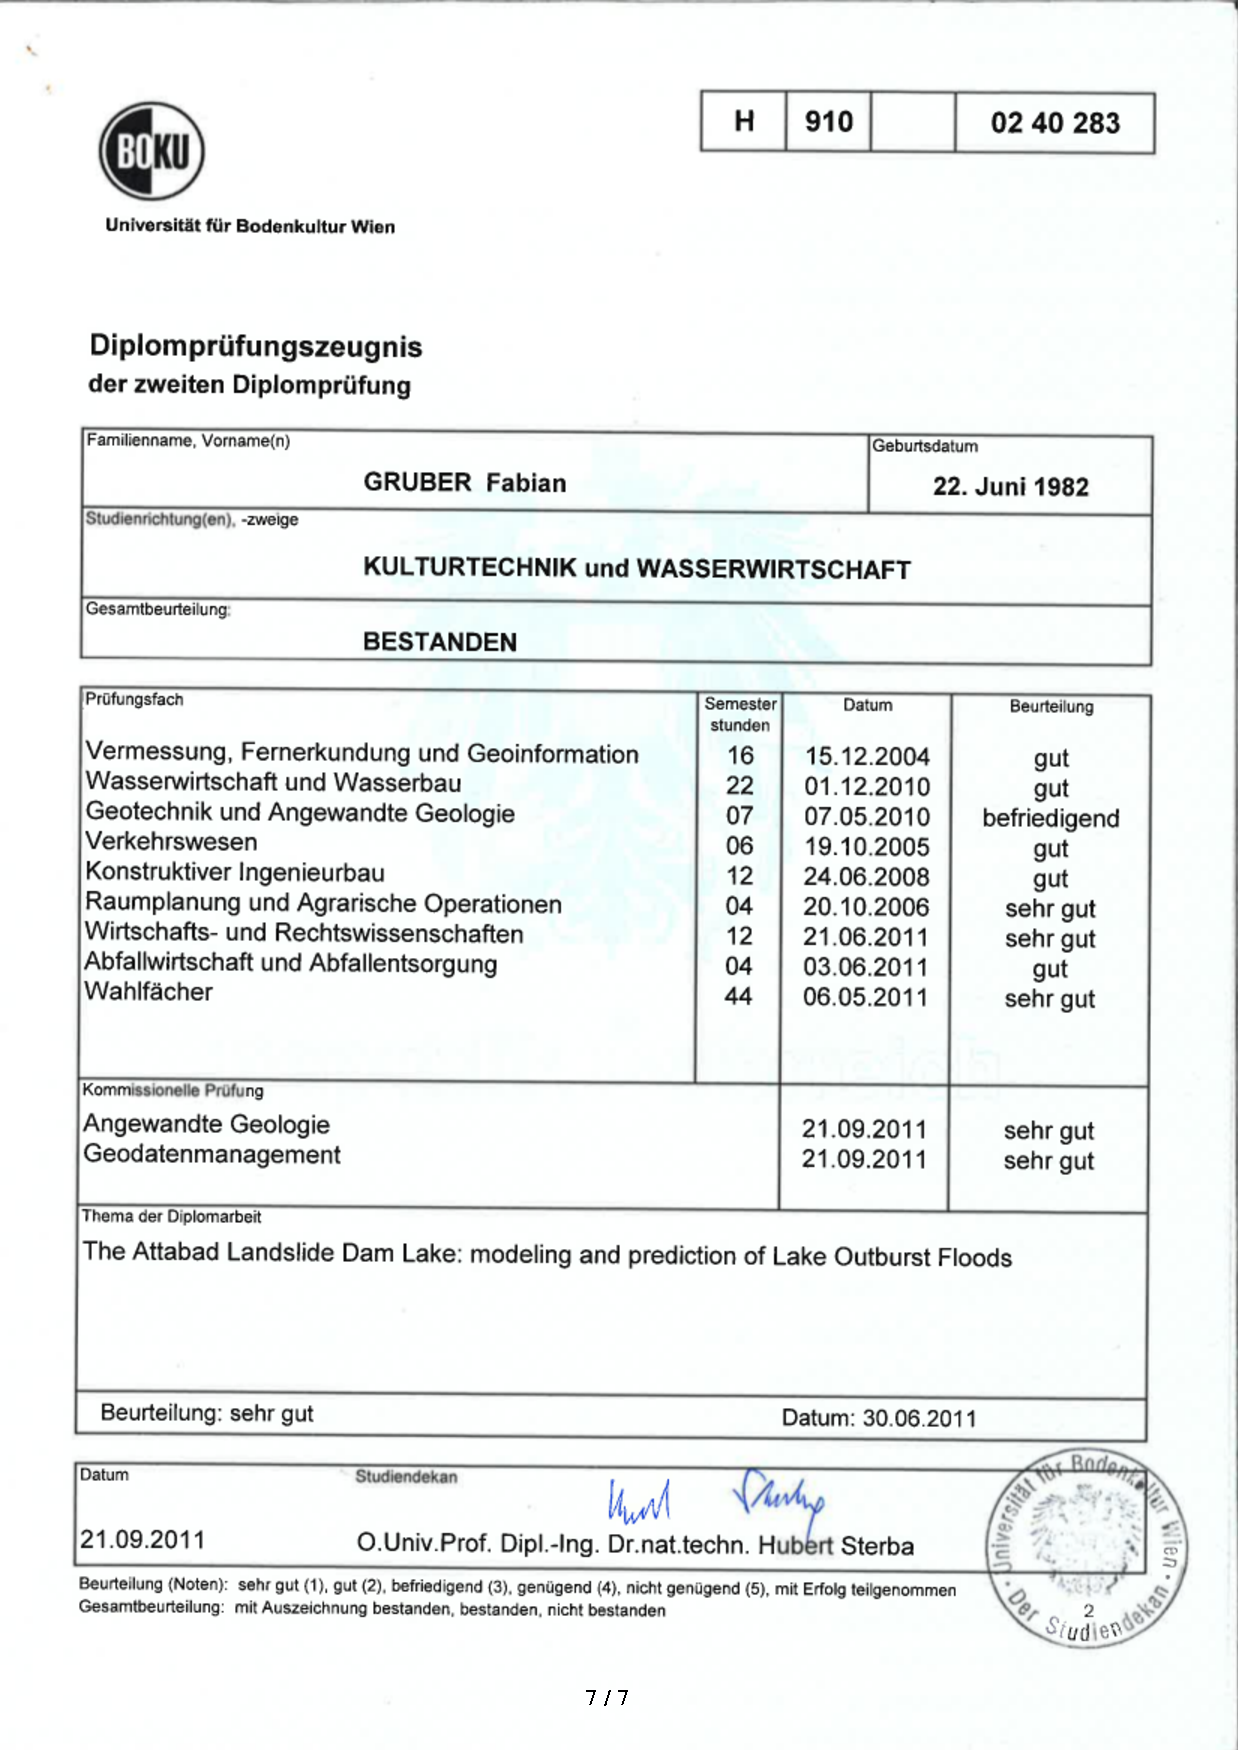
\includepdf{DP1_7von7.pdf}
%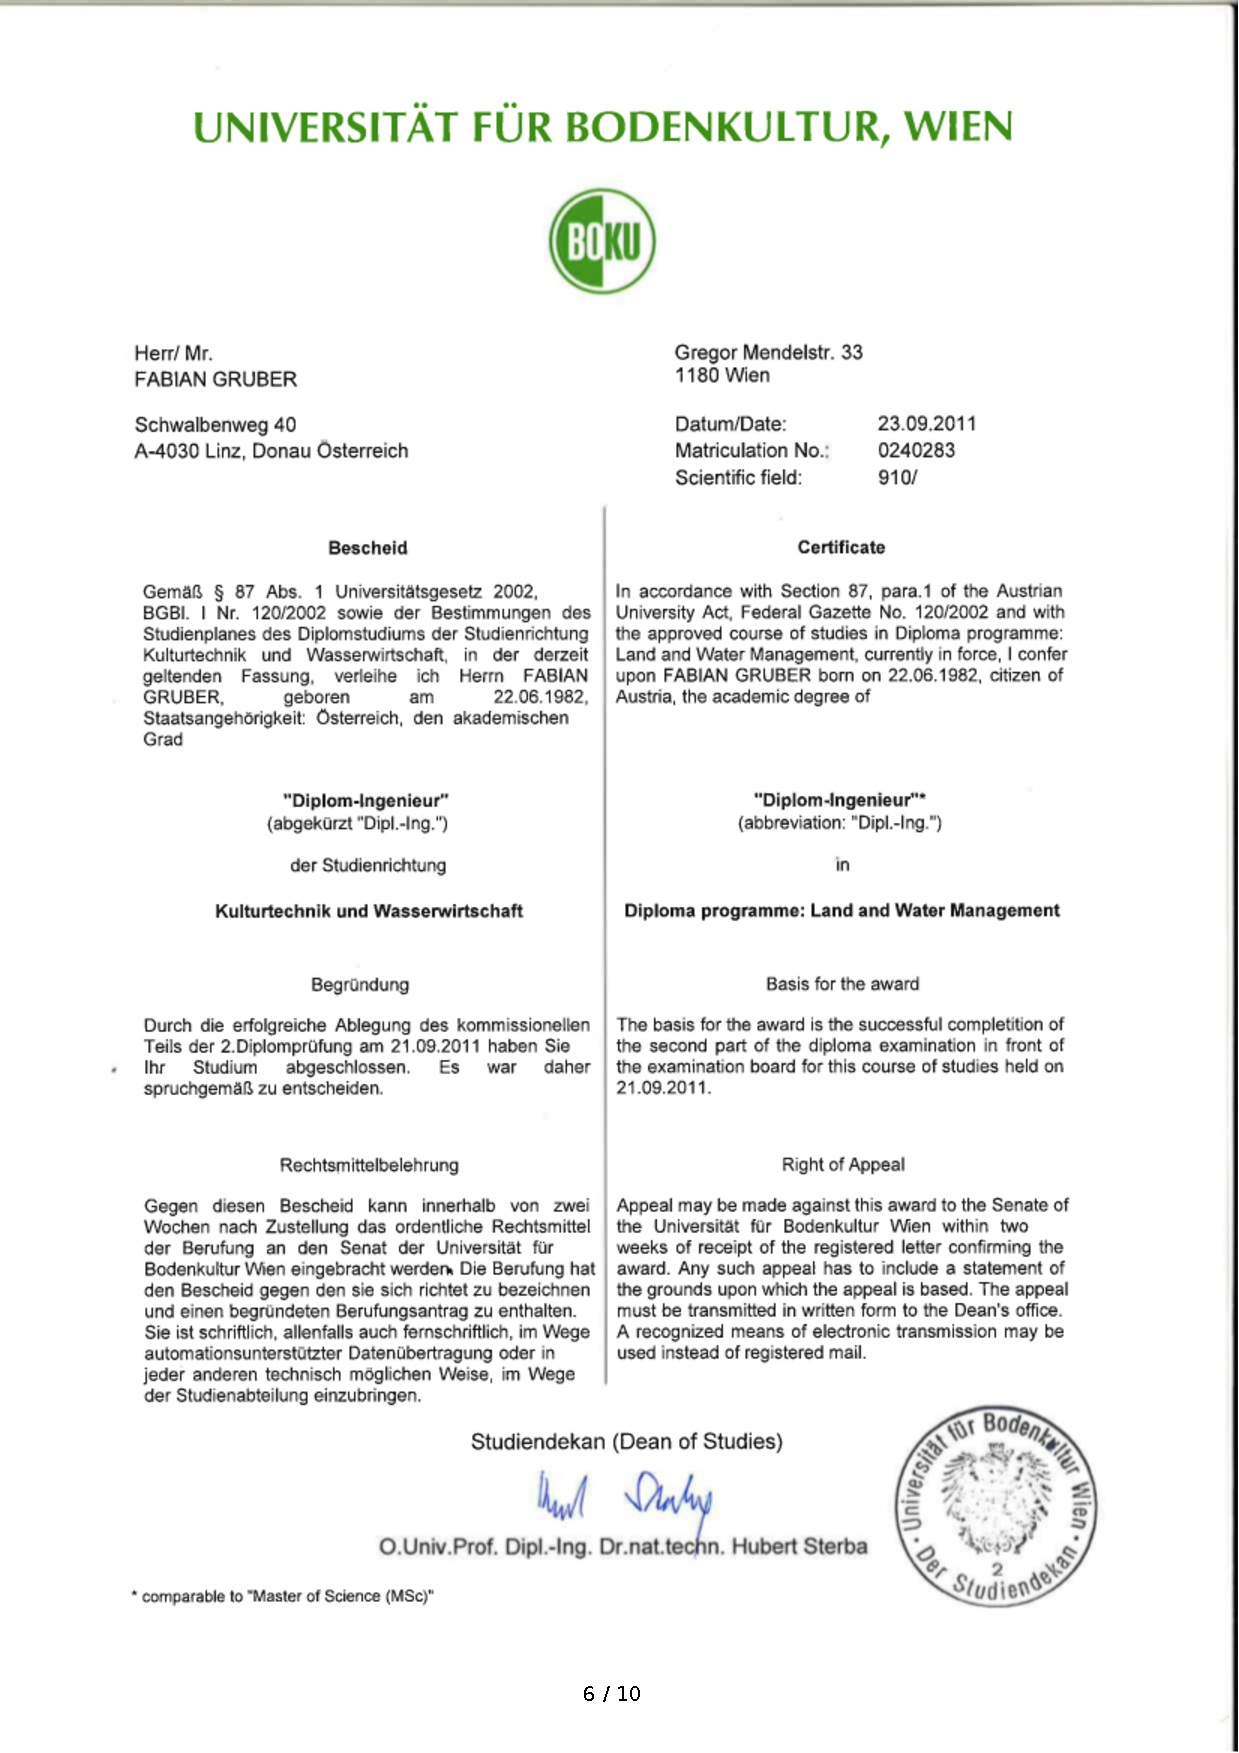
\includepdf{DP_6.pdf}
%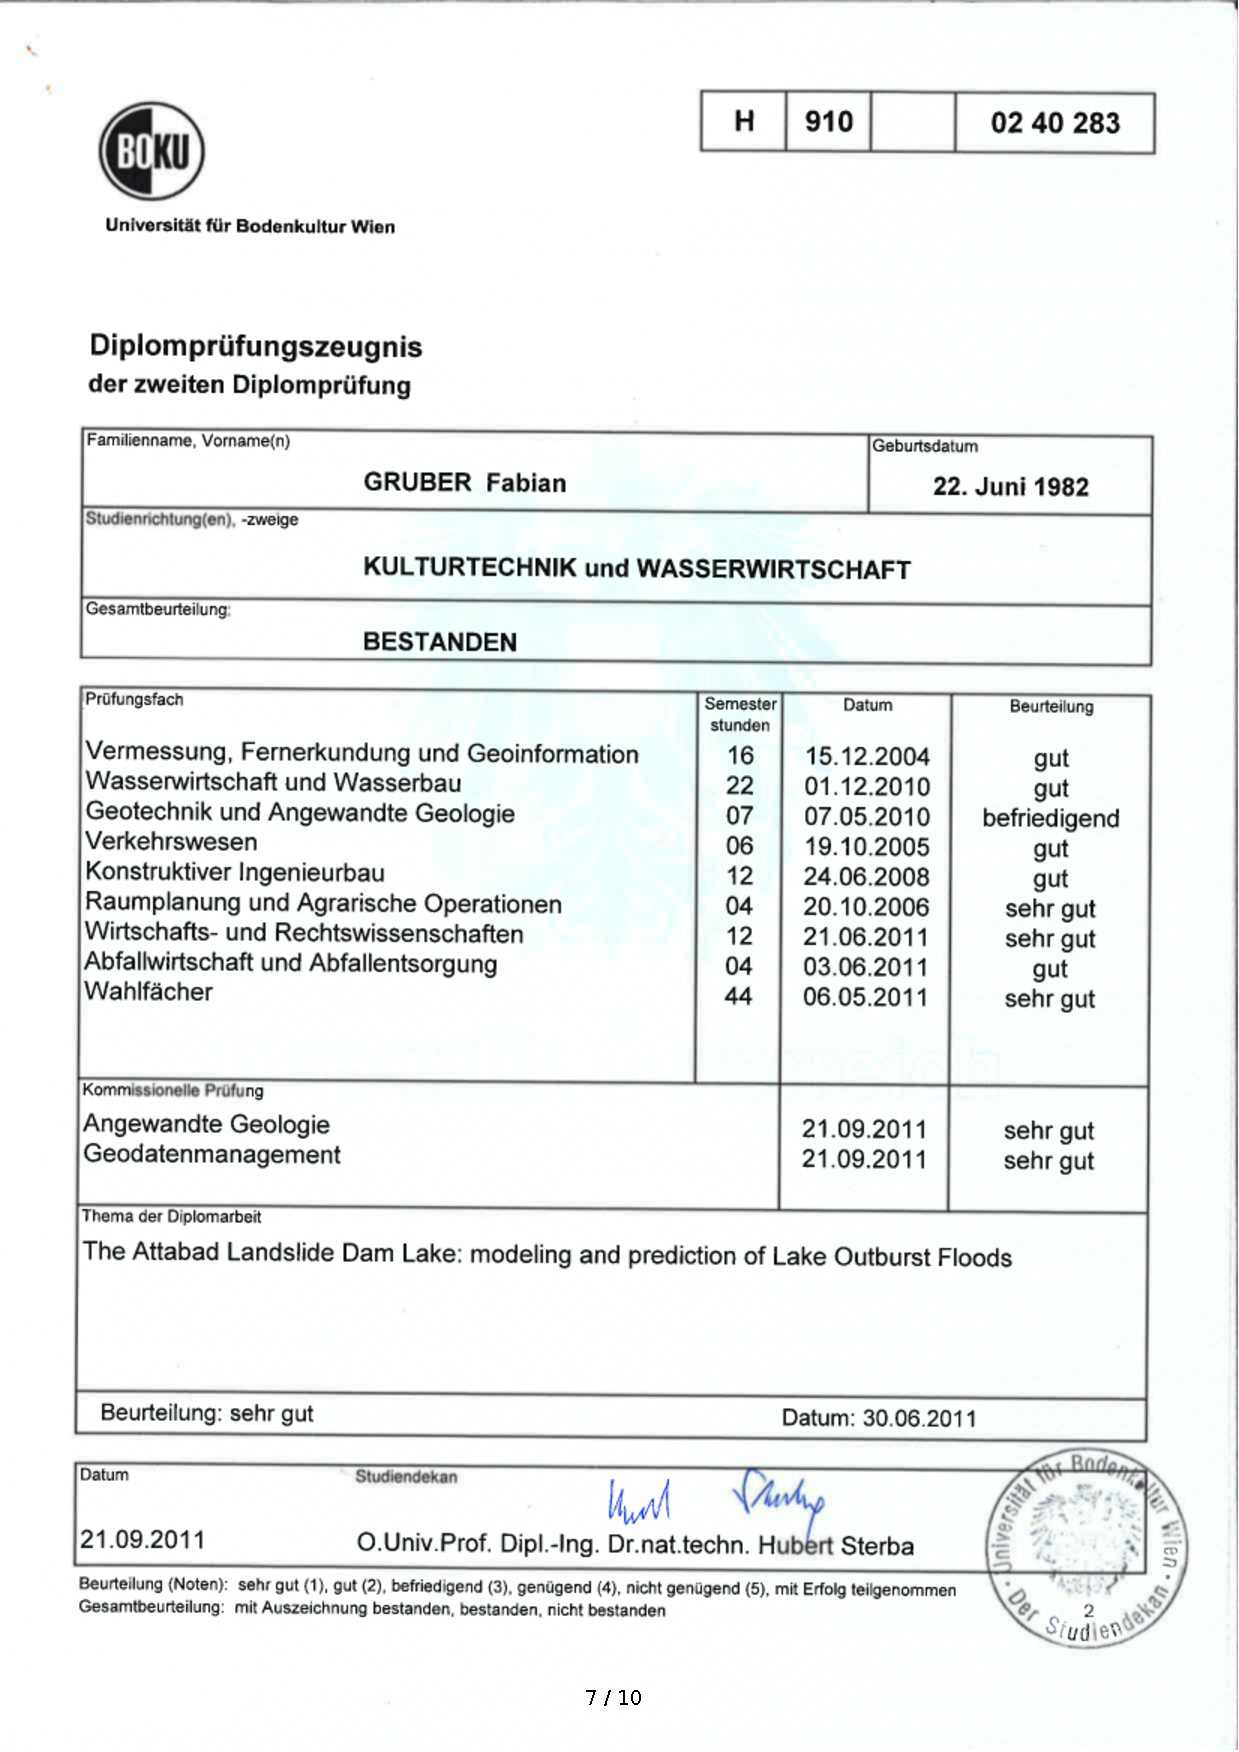
\includepdf{DP1_7.pdf}
%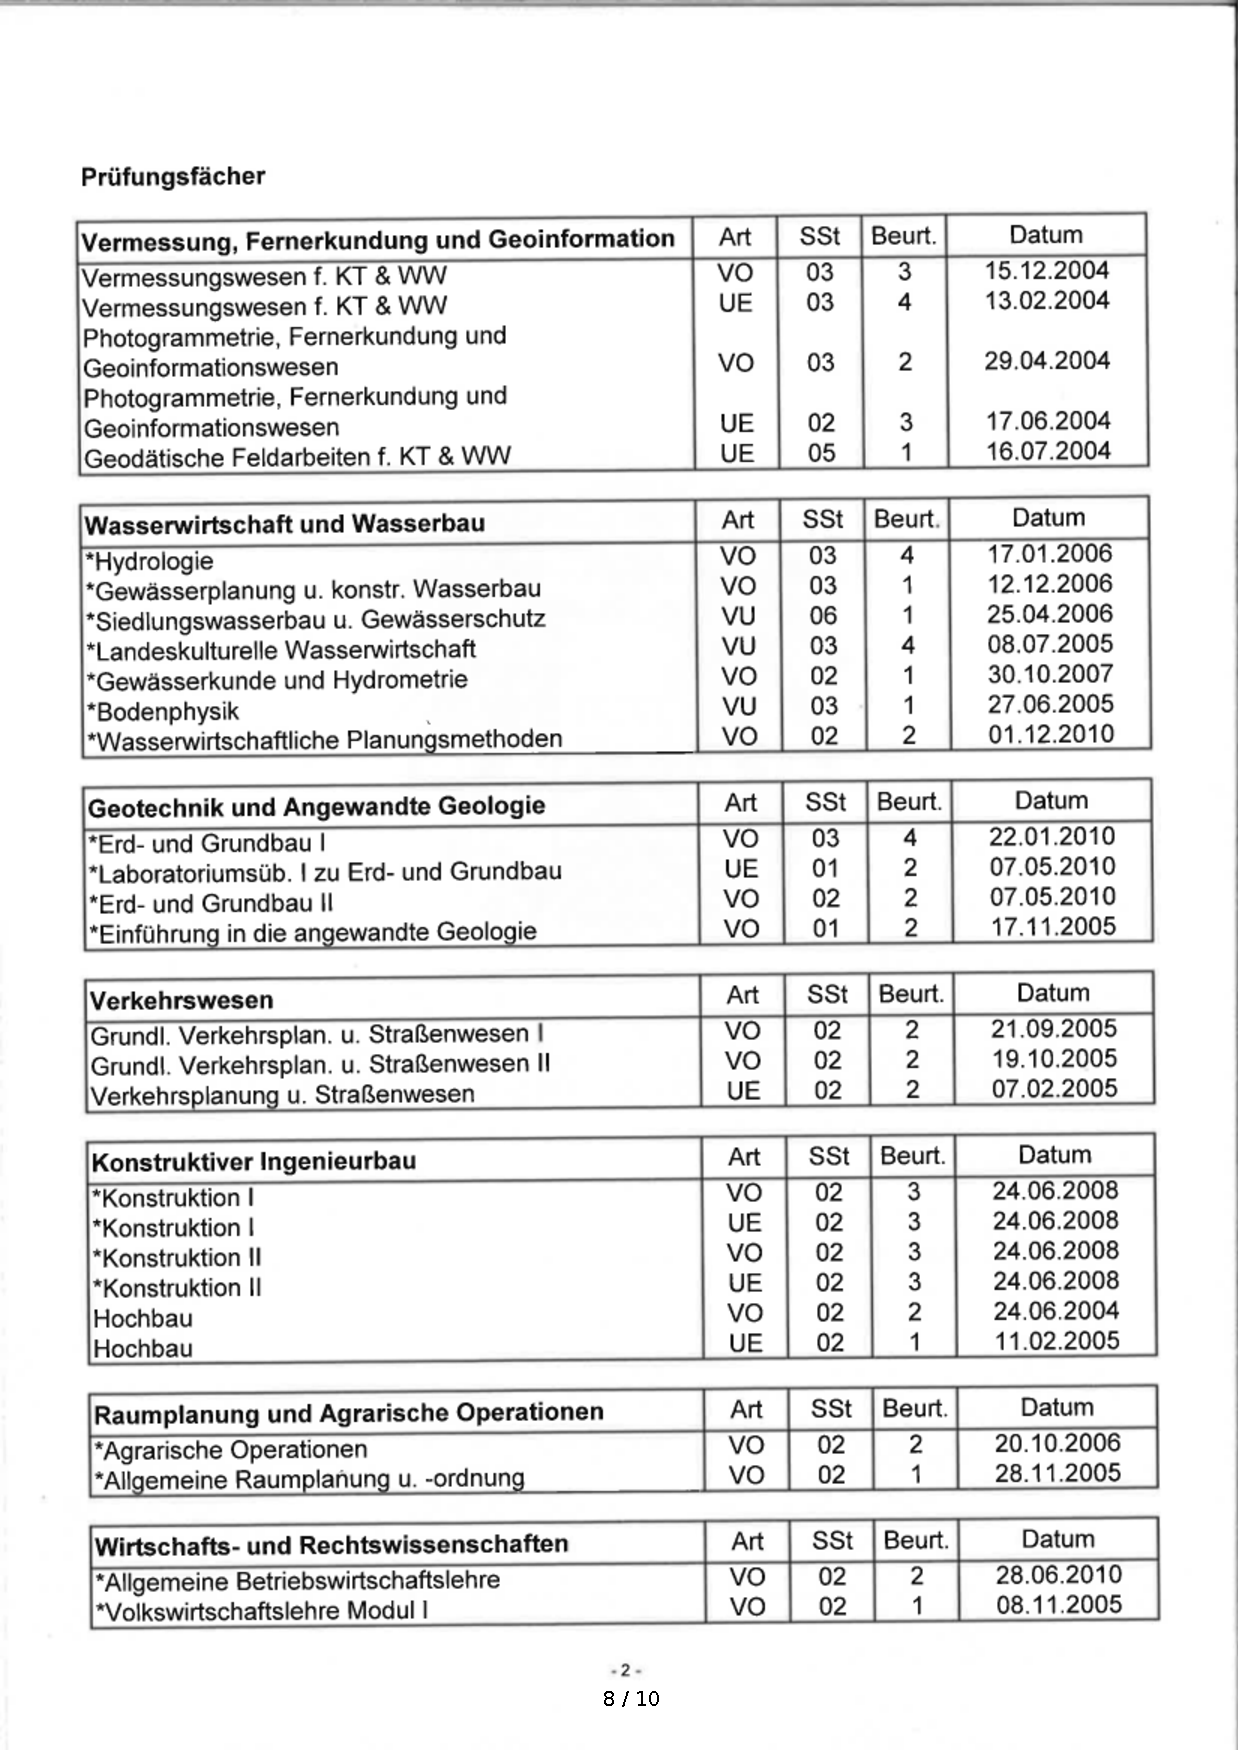
\includepdf{DP2_8.pdf}
%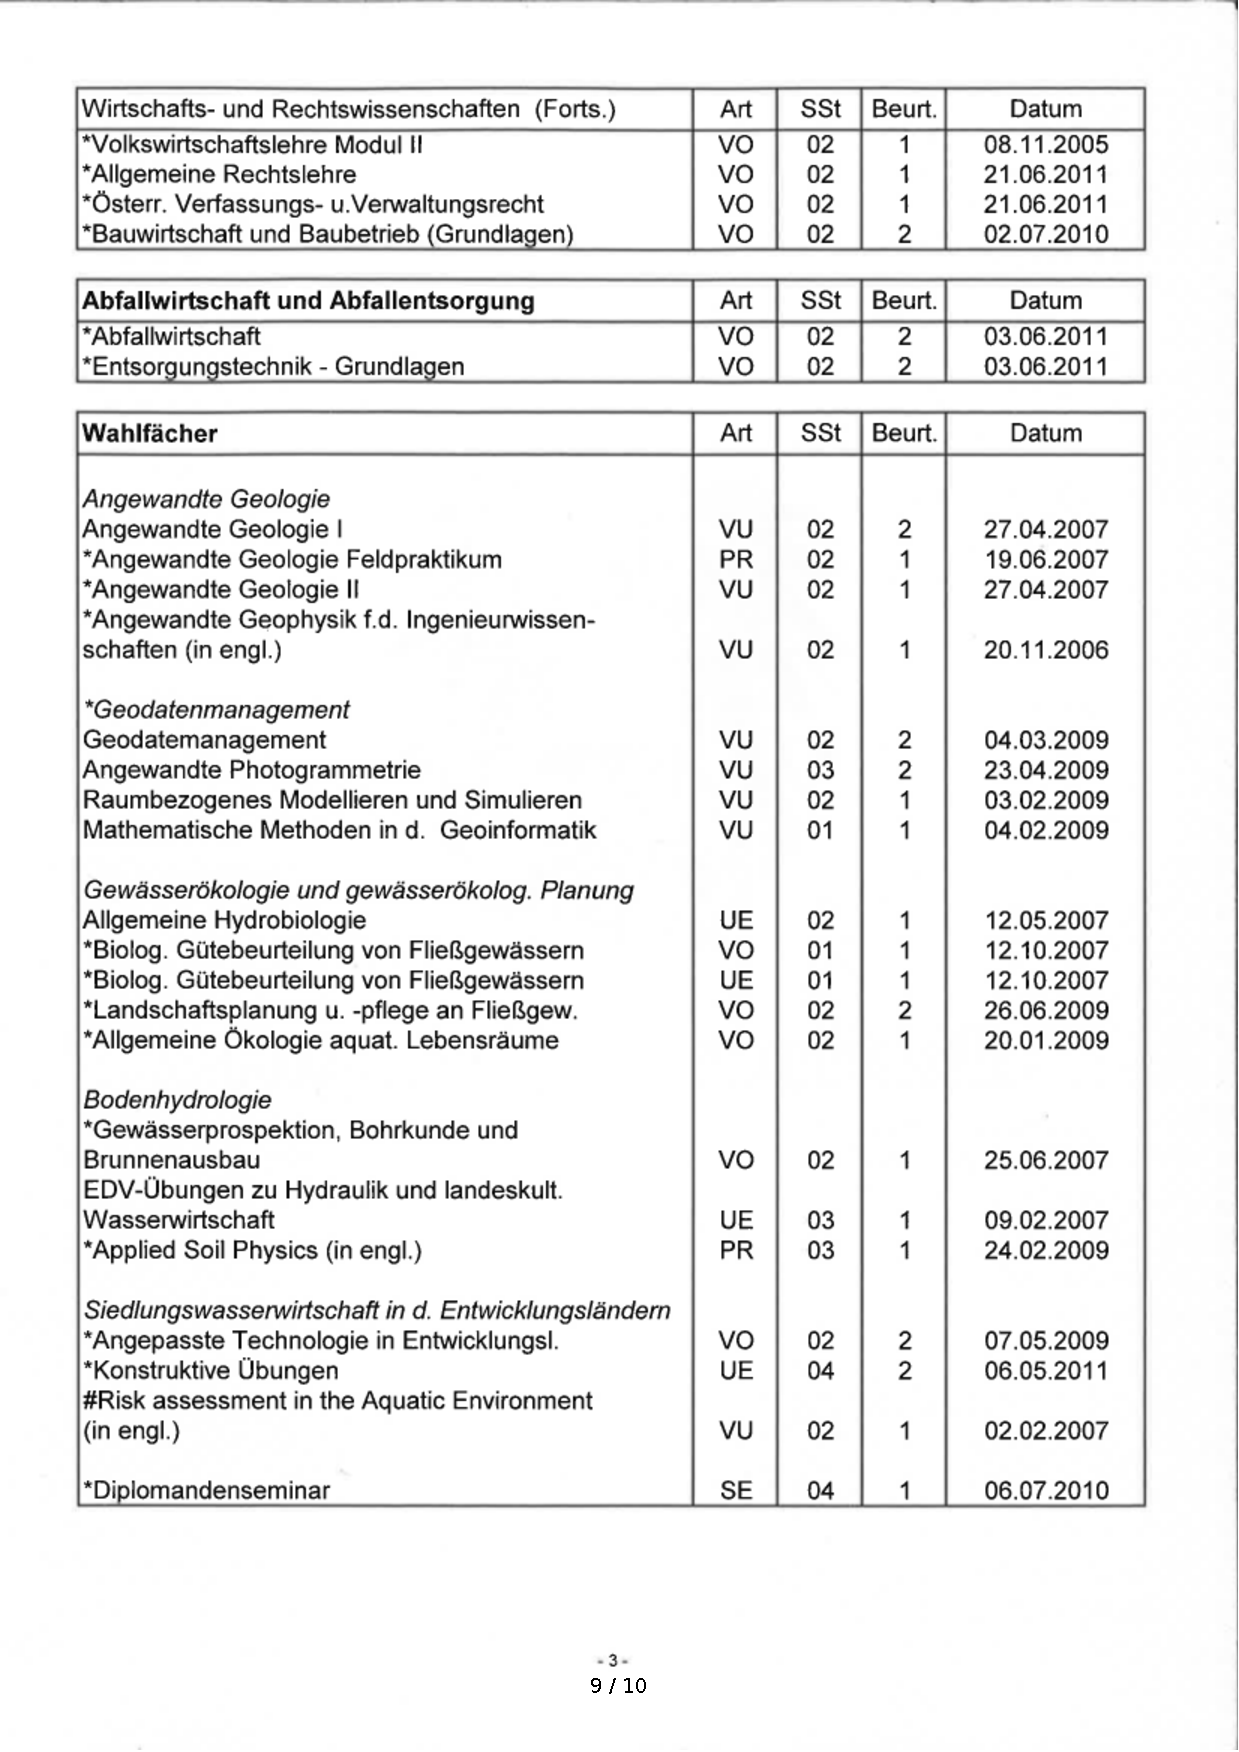
\includepdf{DP3_9.pdf}
%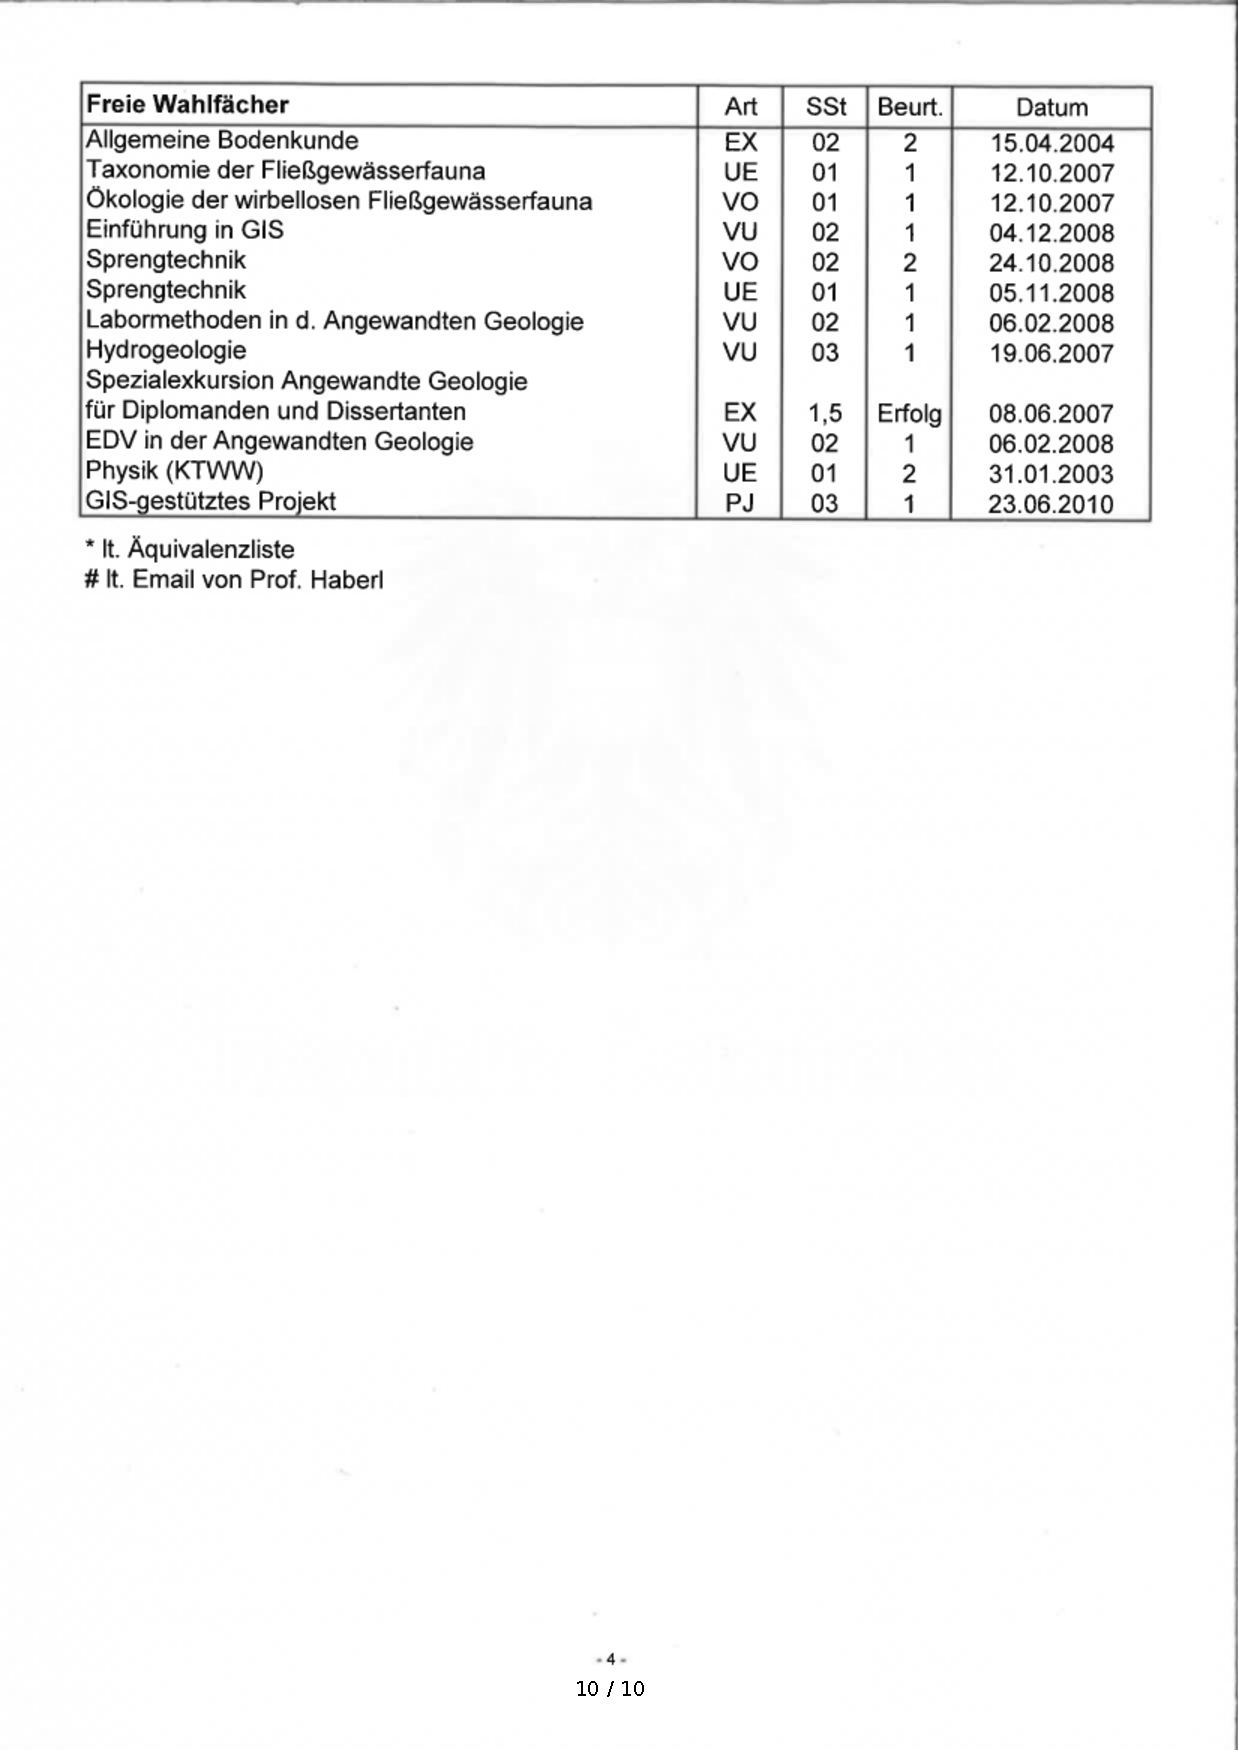
\includepdf{DP4_10.pdf}
\end{document}


%% end of file `template.tex'.
